\documentclass[openany]{book}

\usepackage[a4paper,margin=4.72cm]{geometry}
\usepackage{graphicx}
\usepackage[version=3]{mhchem}
\usepackage{siunitx} 
\usepackage{natbib}
\usepackage{graphicx}
\usepackage{mathtools}
\usepackage{amssymb}
\usepackage{amsthm}
\usepackage[italian]{babel}
\usepackage{stackengine}
\usepackage{graphicx,ifthen}
\usepackage{amsmath}
\usepackage{hyperref}
\usepackage{upgreek}
\usepackage{bm}
\usepackage{braket}
\usepackage{float}
\usepackage{fancyhdr}
\usepackage{appendix}

\makeatletter
\renewcommand{\@chapapp}{Esperienza}
\makeatother

\setcounter{tocdepth}{0}
\makeindex
\title{\textbf{ESPERIMENTAZIONI II: \\ MONOGRAFIE \\ ELETTROTECNICA}}
\author{Manuel Gabriele Moretti}
\date{Settembre 2024}

\begin{document}

\maketitle
\pagenumbering{roman}
\tableofcontents
\newpage

\pagenumbering{arabic}
\chapter{Caratteristica I-V di una lampadina}

\renewcommand\thesection{\Roman{section}}

\section{Resistenze interne di due tester}
\textbf{Obiettivo:} ricavare la resistenza interna di un tester digitale e di un tester analogico.

\paragraph{Strumentazione:}
\begin{enumerate}
    \item un alimentatore di tensione continua;
    \item una resistenza di $\SI{470}{\kilo\Omega}\pm5\%$;
    \item un tester digitale e un tester analogico.
\end{enumerate}

\paragraph{Procedura:}
\begin{enumerate}
    \item accendere il generatore di tensione e cortocircuitarlo impostando la corrente massima erogabile dal generatore a $\SI{0.1}{A}$;
    \item spegnere il generatore e impostare il tester digitale su volt. Per il tester analogico, impostarlo sul fondo scala $\SI{10}{V}$;
    \item Costruire sulla basetta di plexiglas il circuito;
    \begin{figure}[h]
        \centering
        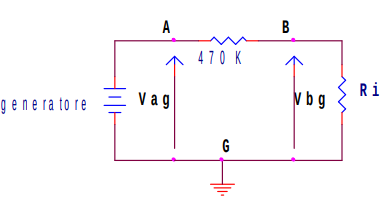
\includegraphics[width=0.5\linewidth]{Immagini/EXP1 - circuito strumenti misura.png}
        \caption{circuito per la misura  delle resistenze interne.}
        \label{fig: EXP1 - circuito strumenti misura}
    \end{figure}
    \item prima di dare tensione ricordare che il tester analogico di cui si dispone non ha protezioni quindi una manovra errata può portare al danneggiamento del tester.
    \item accendere l'alimentatore e regolarlo su circa $\SI{8}{V}$, leggere la tensione $V_{bg}$ con il tester
    \item scollegare il tester e misurare la tensione $V_{ag}$ con il tester.
    \item determinare la resistenza interna $R_i$ corredata della sua incertezza con
    \begin{equation}
        \frac{V_{ag}R_i}{470\times10^3+R_i}=V_{bg};
    \end{equation}
    \item ripetere la misura usando il tester digitale.
\end{enumerate}

\section{Caratteristica I-V di una lampadina}

\paragraph{Obiettivo:} ricavare la caratteristica I-V di una lampadina e verificare la validità della legge di corpo nero per un filamento di tungsteno riscaldato.

\paragraph{Strumentazione:}
\begin{enumerate}
    \item un alimentatore di tensione continua;
    \item una lampadina ad incandescenza;
    \item un tester digitale da usare come voltmetro e un altro da usare come amperometro.
\end{enumerate}

\paragraph{Procedura:}
\begin{enumerate}
    \item misurare la resistenza della lampadina a freddo;
    \item costruire il circuito;
    \begin{figure}[h]
        \centering
        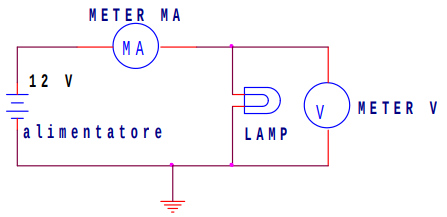
\includegraphics[width=0.6\linewidth]{Immagini/EXP1 - IV lampadina.png}
        \caption{circuito per la I-V della lampadina.}
        \label{fig:EXP1 - IV lampadina}
    \end{figure}
    \item variare il valore di tensione $V_{in}$ fornito dal generatore, da 0 V a 12 V, a passi di 0.5 V. Per ogni valore di tensione $V_{in}$, effettuare una misura di corrente e di tensione ai capi della lampadina. Si devono effettuare tutte le misure in una volta, in progressione ordinata;
    \item ricavare la resistenza della lampadina e la potenza dissipata;
    \item disegnare le funzioni $I(V)$, $R(V)$ e $P(R)$ ed effettuare una regressione sulle ultime due per determinare il valore di $q$; 
    \item i modelli da provare per le regressioni sono $f=aR^4$, $f=a(R^4-b^4)$ e $f=k(T-T_0)+c(T^4-T_0^4)$;
    \item determinare il range di validità di ogni modello.
\end{enumerate}

\setcounter{section}{0}
\renewcommand\thesection{\Alph{section}}

\section{Parametrizzazione \texorpdfstring{$I(V)$}{I(V)}}
Per alcuni materiali, come il tungsteno (metallo di transizione), una buona
rappresentazione dei dati sperimentali si ottiene invece con la relazione
\begin{equation}
    R=R_0\left(\frac{T}{T_0}\right)^b\quad\therefore\quad T=\beta R^{\gamma}.
\end{equation}
Più $\gamma$ è diverso dal valore unitario, meno la relazione tra T ed R si può approssimare da una proporzionalità diretta.

La lampadina consuma la potenza $P=VI$, dissipata in una piccola parte per via
conduttiva e convettiva, $k(T-T_0)$, e per la maggior parte per via radiativa, secondo la legge di corpo nero $P=e\sigma A_s(T^4-T_0^4)$. In prima approssimazione si può trascurare $T_0$ in quanto $T_{filamento}\approx\SI{2000}{\celsius}$. Quindi si ha
\begin{equation}
    P=VI=cT^4=c(\beta R^{\gamma})^4=mR^q,\quad q=4\gamma.
\end{equation}
Ricordando che $R=V/I$ si trova
\begin{equation}
    I=\sqrt[q+1]{m}V^{\frac{q-1}{q+1}}=sV^{\frac{q-1}{q+1}}.
\end{equation}
\chapter{Ciclo di isteresi}

\renewcommand\thesection{\Roman{section}}

\textbf{Obiettivo:} Determinare i rapporti di trasformazione, visualizzare il ciclo di isteresi dei lamierini magnetici componenti un trasformatore e determinare la resistenza interna di un oscilloscopio.

\paragraph{Strumentazione:} 
\begin{enumerate}
    \item il circuito pre-costruito con i trasformatori;
    \item una resistenza di circa $\SI{500}{\kilo\Omega}$ e un condensatore di capacità tale che $RC\gg T=\SI{20}{ms}$;
    \item un oscilloscopio.
\end{enumerate}

\paragraph{Procedura:}
\begin{enumerate}
    \item usando i due canali dell'oscilloscopio misurare le tensioni delle boccole A e B riferite a G (ground) che rappresenta la massa del sistema;
    \begin{figure}[h]
        \centering
        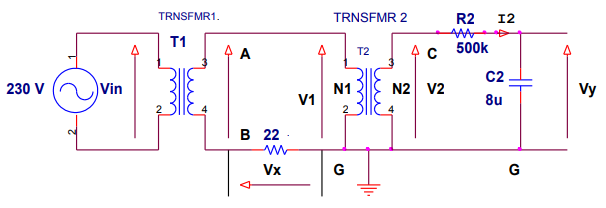
\includegraphics[width=0.8\linewidth]{Immagini/EXP2 - circuito ciclo isteresi.png}
        \caption{circuito per visualizzare il ciclo di isteresi.}
        \label{fig: EXP2 - circuito ciclo isteresi}
    \end{figure}
    \item ricavare la tensione $V_{AB}\sin{\omega t}$ in uscita dal primo trasformatore con le funzioni MATH dell'oscilloscopio, la tensione $V_{AB}$ è il valore massimo;
    \item ricavare il rapporto di trasformazione del primario e del secondario sapendo che
    \begin{equation}
        n_1=\frac{N_{p}}{N_{s}}=\frac{230}{V_{AB,eff}};
    \end{equation}
    \item misurare la tensione $V_{CG}$ e calcolare il rapporto di trasformazione del secondo trasformatore con 
    \begin{equation}
        n_2=\frac{N_p'}{N_s'}=\frac{V_{BG}}{V_{CD}};
    \end{equation}
    \item inserire fra C e D la resistenza, inserire tra D e G il condensatore e misurare la tensione $V_{DG}$;
    \item impostare l'oscilloscopio in funzionamento X-Y ed applicare al canale X la $V_{BG}$ ed al canale Y la $V_{DG}$: si vedrà sullo schermo il ciclo di isteresi;
    \item sostituire il condensatore con l'oscilloscopio e misurare le tensioni $V_{CG}$ e $V_{DG}$;
    \item risolvere per $R_i$ la relazione
    \begin{equation}
        \frac{V_{CG}R_i}{R+R_i}=V_{DG}.
    \end{equation}
\end{enumerate}

\setcounter{section}{0}
\renewcommand\thesection{\Alph{section}}

\section{Visualizzazione del ciclo d'isteresi}
Per visualizzare il ciclo di isteresi di lamierini magnetici componenti un trasformatore, si può usare il circuito in figura \ref{fig: EXP2 - circuito ciclo isteresi}. Scrivendo l'equazione di maglia del primario si ha
\begin{equation}
    v_1 - L_1 \frac{d i_1}{dt} - M\frac{d i_2}{dt} = R_1i_1.
\end{equation}
Ricordando che $Hl=N_1i_1+N_2i_2$, dove $l$ è la lunghezza del circuito magnetico, si ha che $H\propto N_1i_1\propto i_1R_1 \propto v_{R_1}=v_X$. Nel circuito del secondario si ha
\begin{equation}
    v_2 = N_2 \frac{d\Phi}{dt} = N_2S\frac{dB}{dt}m\quad\therefore\quad dB=\frac{v_2}{N_2S}dt,
    \label{placeholder_label}
\end{equation}
la quale integrata restituisce
\begin{equation}
    B=\frac{1}{N_2S}\int v_2dt+C=\frac{1}{N_2S}v_y+C.
\end{equation}
Inviando sul canale X dell'oscilloscopio la tensione $v_x$ e sul canale Y la tensione $v_y$ si ottiene disegnato sullo schermo il ciclo di isteresi.
\chapter{Circuiti RC}

\renewcommand\thesection{\Roman{section}}

\section{Filtri RC}
\textbf{Obiettivo:} verificare il tipo di circuito, ricavare il rapporto di amplificazione del circuito e confrontare il valore della frequenza di taglio. 

\paragraph{Strumentazione:} 
\begin{enumerate}
    \item un alimentatore di tensione continua;
    \item una resistenza e un condensatore tali che la frequenza di taglio $f_0$ del circuito sia di qualche kHz;
    \item un voltmetro.
\end{enumerate}

\paragraph{Procedura:}
\begin{enumerate}
    \item costruire un circuito passa basso e un circuito passa alto scambiando la resistenza con il condensatore;
    \begin{figure}[h]
        \centering
        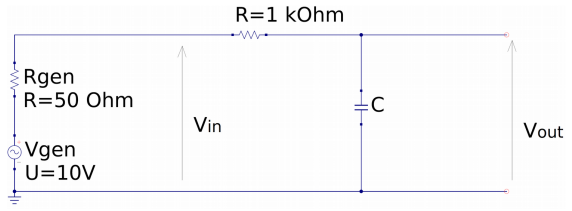
\includegraphics[width=0.6\linewidth]{Immagini/EXP3 - passabasso.png}
        \caption{filtro passa basso.}
        \label{fig: EXP3 - passabasso}
    \end{figure}
    \item misurare con l'oscilloscopio la tensione all'ingresso del circuito e all'uscita per varie frequenze;
    \item graficare il rapporto delle tensioni in funzione della frequenza;
    \item verificare che è un circuito passa alto o passa basso, effettuando una regressione;
    \item effettuare questa parte dell'analisi senza utilizzare le misure di R e C, ossia lavorando come se il quadrupolo fosse di costruzione incognita;
    \item confrontare il valore della frequenza di taglio ottenuta dalla regressione dei dati con il valore che si ottiene dalla misura di R e C. 
\end{enumerate}

\section{Derivatori ed integratori}

\textbf{Obiettivo:} verificare che i circuiti RC passa alto e passa basso sono funzionano anche come circuiti derivatori e integratori.

\paragraph{Procedura:}
nel caso di un passa alto l'equazione di maglia è $V_{in}=V_{out}+V_C$, dove 
\begin{equation}
    V_C=\frac{1}{C}\int idt+C,
\end{equation}
mentre ai capi della resistenza R si ha $V_{out}=Ri$, quindi l'equazione di maglia diventa
\begin{equation}
    V_{in}=V_{out}+\frac{1}{RC}\int V_{out}dt+C,
\end{equation}
dove se $V_{out}$ è trascurabile si ha
\begin{equation}
    V_{in}=\frac{1}{RC}\int V_{out}dt+C,
\end{equation}
la quale derivata restituisce
\begin{equation}
    V_{out}=RC\frac{dV_{in}}{dt}.
\end{equation}
La condizione necessaria è che $V_{out}$ sia trascurabile. Questa condizione si può ottenere se la costante di tempo RC è molto piccola rispetto al periodo della funzione d'onda in ingresso.
\begin{enumerate}
    \item Calcolare e poi verificare sperimentalmente il valore di R necessario per avere, alla frequenza di 1 kHz uno sfasamento fra tensione di ingresso ed uscita vicino a 90°;
    \item applicando delle onde quadre all'ingresso del circuito verificare sotto quali condizioni il circuito effettua la funzione di derivata;
    \item provare ad inviare un'onda triangolare ed osservare la tensione in uscita. 
\end{enumerate}
Nel caso di un passa basso l'equazione di maglia è $V_{in}=V_R+V_C=Ri+V_{out}$, ma derivando l'equazione di $V_C$ e sostituendola in questa equazione si ha
\begin{equation}
    V_{in}=RC\frac{dV_{out}}{dt}+V_{out}.
\end{equation}
Ipotizzando di poter trascurare $V_{out}$ ed integrando si ottiene
\begin{equation}
    V_{out}=\frac{1}{RC}\int V_{in}dt+C.
\end{equation}
La condizione per cui $V_{out}$ è trascurabile si può ottenere usando una costante di tempo RC grande rispetto al periodo della funzione d'onda in ingresso.
\begin{enumerate}
    \item Verificare sperimentalmente che, inviando con il generatore di funzioni un'onda quadra, si può ottenere l'integrale della tensione di ingresso. Si dovrebbe ottenere un'onda triangolare.
    \item Provare ad inviare un'onda triangolare e osservare la tensione in uscita.
\end{enumerate}

\setcounter{section}{0}
\renewcommand\thesection{\Alph{section}}

\section{Guadagno di un filtro RC}
Un circuito RC è un quadripolo composto da due elementi passivi (detti anche bipoli): una resistenza che ha un comportamento costante con il variare della frequenza; ed un condensatore la cui impedenza varia con l'inverso della frequenza. Usando il calcolo simbolico (applicabile solo se il segnale di ingresso è sinusoidale) si ha
\begin{equation}
    I = \frac{V_{in}}{R + (j\omega C)^{-1}}.
\end{equation}
Quindi, per il passa alto\footnote{Per il passa basso invece si ha $V_{out}=I/(j\omega C)$.}, si ha
\begin{equation}
 V_{out} = IR = \frac{V_{in}}{R + (j\omega C)^{-1}} R = \frac{V_{in}}{1 + (j\omega RC)^{-1}},
\end{equation}
facendone il modulo si ha 
\begin{equation}
    \left| V_{out} \right| = \frac{\left| V_{in} \right|}{\sqrt{1 + (\omega^2 R^2 C^2)^{-2}}}.
    \label{eq:placeholder}
\end{equation}
Sostituendo $RC=1/(2\pi f_0)$ si ottiene
\begin{equation}
A_V=\left| \frac{V_{out}}{V_{in}} \right| = \frac{1}{\sqrt{1 + f_0^2/f^2}} = \frac{f}{\sqrt{f^2 + f_0^2}},
\end{equation}
dove $A_V$ è il guadagno del quadripolo. \'E utile definire una frequenza limite. La convenzione è la frequenza $f = f_0$, dove il guadagno $A_V$ si riduce a
\begin{equation}
    |A_{VL}|=\frac{1}{\sqrt{2}},
\end{equation}
dove il pedice ``L'' sta per ``low'' cioè la minima frequenza che passa. La fase tra la tensione in uscita e quella in ingresso si ottiene da
\begin{equation}
\frac{V_{out}}{V_ {in}} = \frac{1}{1 + (\omega^2 R^2 C^2)^{-1}}\left(1 + \frac{j}{\omega RC}\right)\Rightarrow\tan{\phi}=\frac{1}{\omega RC}.
\end{equation}
Sostituendo $f_0$ si ha $\tan{\phi}=f_0/f$ e se $f=f_0$ si ha $\tan{\phi}=1\Rightarrow\phi=45$°.
Riassumendo:
\begin{itemize}
    \item per frequenze minori di $f_0$ il segnale di ingresso per convenzione non passa in uscita;
    \item per $f = f_0$ il segnale di uscita è $\sqrt{2}$ volte minore del segnale di ingresso e la tensione di uscita è di 45° in anticipo rispetto a quella di ingresso.
\end{itemize}

\chapter{Circuiti RLC}

\renewcommand\thesection{\Roman{section}}

\section{Rifasamento}

\textbf{Obiettivo:} minimizzare lo sfasamento tra tensione e corrente in un circuito RL tramite l'aggiunta in serie di un condensatore.

\paragraph{Strumentazione:}
\begin{enumerate}
    \item un generatore di funzioni;
    \item una resistenza;
    \item un induttore;
    \item un oscilloscopio.   
\end{enumerate}

\paragraph{Procedura:}
\begin{enumerate}
    \item costruire il circuito;
    \begin{figure}[h]
        \centering
        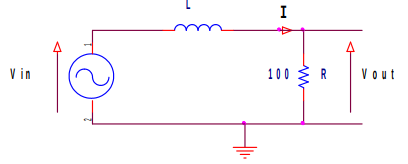
\includegraphics[width=0.6\linewidth]{Immagini/EXP4 - circuito RL.png}
        \caption{serie RL da rifasare.}
        \label{fig: EXP4 - circuito RL}
    \end{figure}
    \item misurare il valore di L e di Q (fattore di bontà);
    \item usando un generatore di funzioni applicare una tensione sinusoidale al circuito e con l'oscilloscopio visualizzare la tensione applicata all'ingresso e ai capi della resistenza. Si vede con i due canali dell'oscilloscopio che c'è uno sfasamento fra le due tensioni, ed anche fra tensione e corrente;
    \item con i cursori, misurare lo sfasamento tra le due tensioni;
    \item a partire dal valore misurato dell'induttanza, calcolare il condensatore necessario per il rifasamento ad una frequenza di circa 10 kHz;
    \item verificare che le due tensioni sono in fase misurando il loro sfasamento.
    \begin{figure}[h]
        \centering
        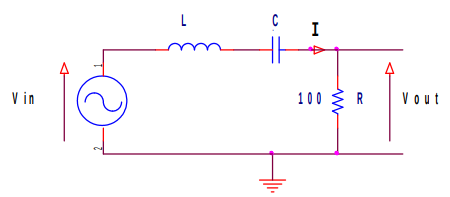
\includegraphics[width=0.55\linewidth]{Immagini/EXP4 - circuito RLC.png}
        \caption{serie RLC rifasata.}
        \label{fig: EXP4 - circuito RLC}
    \end{figure}
\end{enumerate}

\section{Guadagno di un soppressore di banda}

\paragraph{Obiettivo:} ricavare il guadagno di un soppressore di banda (o di un passa banda) in funzione della frequenza della tensione in ingresso.

\paragraph{Strumentazione:} 
\begin{enumerate}
    \item un generatore di funzioni;
    \item una resistenza;
    \item un induttore e un condensatore tali che la frequenza di risonanza $f_0$ sia di qualche kHz;
    \item un oscilloscopio.
\end{enumerate}

\paragraph{Procedura:}
\begin{enumerate}
    \item costruire il circuito;
    \begin{figure}[h]
        \centering
        \includegraphics[width=0.7\linewidth]{Immagini/EXP4 - passa|elimina banda.png}
        \caption{passa banda o soppressore di banda.}
        \label{fig: EXP4 - passa|elimina banda}
    \end{figure}
    \item collegare il generatore di funzioni, impostato su onde sinusoidali, all'ingresso del circuito;
    \item per eseguire la misura collegare un canale dell'oscilloscopio all'ingresso e l'altro all'uscita;
    \item per frequenze vicine a $f_0$ si avrà una tensione in uscita circa uguale a quella in ingresso (passa banda), oppure una tensione prossima a zero (soppressore di banda);
    \item caratterizzare la risposta del filtro in funzione della frequenza, misurando per ogni valore la tensione di ingresso e in uscita. Per caratterizzarlo al meglio, oltre a prendere misure nell'intorno di $f_0$, prenderne anche per valori di $f$ molto minori e molto maggiori di $f_0$;
    \item graficare il guadagno $A_V$ in funzione di $f$;
    \item verificare che cambiando il valore della resistenza del circuito la banda passante si restringe o si allarga;
    \item dopo aver ricavato mediante calcolo simbolico il guadagno in funzione di $f$, effettuare una regressione dei dati con la relativa funzione. Confrontare la frequenza di risonanza ottenuta dal fit con quella ricavabile dalle misure di L e C. Per l'inizializzazione dei parametri della funzione di fit utilizzare solo le informazioni ricavabili dai dati e non quelle su L e C. Dal fit estrarre il valore di $R_s$.
\end{enumerate}

\setcounter{section}{0}
\renewcommand\thesection{\Alph{section}}

\section{Corrente attraverso una serie RLC}
Se il generatore è di tipo sinusoidale si può applicare il metodo simbolico per il calcolo della corrente $I$ e si ottiene
\begin{equation}
  I = \frac{V_{in}}{R + j\omega L} = \frac{V_{in}}{R^2 + \omega^2 L^2}(R - j \omega L),
\end{equation}
da cui si ricava
\begin{equation}
    |I| = \frac{V_{in}}{\sqrt{R^2 + \omega^2 L^2}},\quad\tan{\phi}=\frac{-\omega L}{R},
\end{equation}
dove il segno meno indica che la corrente è in ritardo rispetto alla tensione. Per rifasare il circuito è necessario aggiungere un condensatore in serie ad $L$. La corrente diventa
\begin{equation}
I = \frac{V_{in}}{R + j\omega L - \frac{j}{\omega C}} = \frac{V_{in}}{R + j\left( \omega L - \frac{1}{\omega C} \right)}.
\end{equation}
Questa è in fase se $X_L=\omega L=1/(\omega C)=X_C$, da cui si può ricavare il valore di C. In questo caso l'impedenza $Z$ è puramente reale e resistiva.
\chapter{Diodi}

\renewcommand\thesection{\Roman{section}}

\section{Caratteristica I-V di un diodo}

\textbf{Obiettivo:} ricavare le caratteristiche I-V di un diodo al silicio e di un diodo LED.

\paragraph{Strumentazione:}
\begin{enumerate}
    \item un generatore di tensione;
    \item un diodo al silicio e un diodo LED;
    \item una resistenza tra $\SI{0.5}{\kilo\Omega}$ e $\SI{5}{\kilo\Omega}$;
    \item un amperometro e un voltmetro.
\end{enumerate}

\paragraph{Procedura:}
\begin{enumerate}
    \item costruire il circuito;
    \begin{figure}[h]
        \centering
        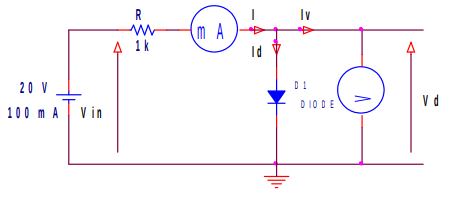
\includegraphics[width=0.6\linewidth]{Immagini/EXP5 - IV diodo.png}
        \caption{circuito da costruire}
        \label{fig: EXP5 - IV diodo}
    \end{figure}
    \item per il diodo al silicio, variare la tensione in ingresso e costruire il grafico di $I(V_d)$, dove $V_d$ è la tensione del diodo;
    \item effettuare una regressione dei dati con l'equazione di Shockley
    \begin{equation}
    I_{d} = I_{s} \left( e^{V_{d}/\eta V_{T}} - 1 \right),\quad V_T=\frac{kT}{e}=\SI{26}{mV}.
    \end{equation}
    \item Dai dati sperimentali si può ricavare $\eta$ che per diodi al silicio vale circa 2, per poi diminuire ad alte correnti di conduzione del diodo.
    \item il diodo LED ha invece una componente resistiva non trascurabile, che fa sì che l'equazione di Shockley non descriva bene l'andamento della corrente ad alti valori. Ai capi del diodo è presente una caduta di potenziale $V_{d} = R_dI_d$. Non è possibile ricavare l'espressione analitica di $I_d(V_d)$, ma è possibile ricavare $V_d(I_d)$, invertendo la relazione di Shockley ed aggiungendo il termine resistivo
    \begin{equation}
        V_d=\eta V_T\ln{\left(\frac{I_d}{I_s}+1\right)}+R_dI_d.
    \end{equation}
\end{enumerate}

\section{Raddrizzamento di una semionda}

\paragraph{Obiettivo:} rendere la tensione ``pulsata'' costante nel tempo tramite l'aggiunta di un filtro RC.

\paragraph{Strumentazione:}
\begin{enumerate}
    \item un generatore di funzioni;
    \item un diodo al silicio;
    \item un condensatore di $\SI{10}{\micro\farad}$ e una resistenza di $\SI{1}{\kilo\ohm}$ per creare un filtro RC;
    \item un oscilloscopio.
\end{enumerate}

\paragraph{Procedura:}
\begin{enumerate}
    \item applicando all'ingresso di un circuito, con in serie il diodo e una resistenza, una tensione sinusoidale, si può osservare con l'oscilloscopio che la tensione di uscita contiene solo la semionda positiva;
    \begin{figure}[h]
        \centering
        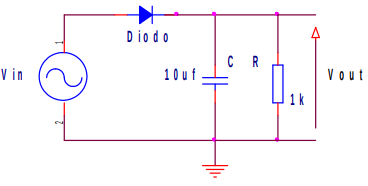
\includegraphics[width=0.6\linewidth]{Immagini/EXP5 - semionda.png}
        \caption{circuito per il raddrizzamento della semionda.}
        \label{fig: EXP5 - semionda}
    \end{figure}
    \item per renderla costante nel tempo si deve aggiungere un condensatore in parallelo alla resistenza, in modo da formare un filtro RC;
    \item verificare l'andamento della tensione in uscita.
\end{enumerate}

\setcounter{section}{0}
\renewcommand\thesection{\Alph{section}}

\section{Modellizzazione di un diodo}
Dalla caratteristica del diodo al silicio si osserva che esso comincia a condurre per tensioni $V_d$ maggiori di 0.5 V ed essendo un andamento esponenziale la corrente sale molto velocemente con la tensione applicata. Con questa osservazione per semplificare i calcoli del circuito, si può sostituirlo con dei modelli in modo da poter applicare la legge di Ohm. Per un diodo ideale:
\begin{itemize}
    \item se conduce, sostituirlo con un cortocircuito;
    \item  se non conduce, sostituirlo con un circuito aperto.
\end{itemize}
\begin{figure}[h]
    \centering
    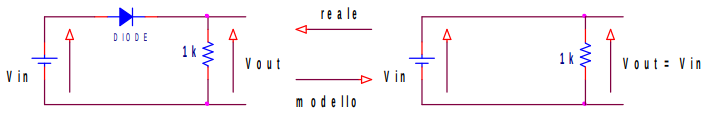
\includegraphics[width=0.9\linewidth]{Immagini/EXP5 - diodo (conduzione).png}
    \caption{diodo in conduzione.}
    \label{fig: EXP5 - diodo (conduzione)}
\end{figure}
\begin{figure}[h]
    \centering
    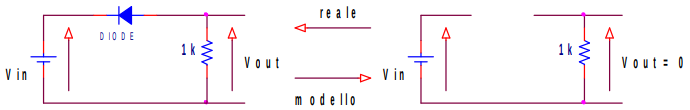
\includegraphics[width=0.9\linewidth]{Immagini/EXP5 - diodo (no conduzione).png}
    \caption{diodo non in conduzione.}
    \label{fig: EXP5 - diodo (no conduzione)}
\end{figure}
Un altro modello molto usato è quello di sostituire il diodo in conduzione con una
resistenza $r_f\approx\SI{10}{\ohm}$ ed un generatore $V_{\gamma}\approx\SI{0.5}{V}$ collegati fra loro in serie
\begin{figure}[h]
    \centering
    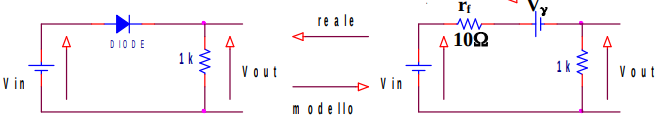
\includegraphics[width=0.9\linewidth]{Immagini/EXP5 - modello diodo (conduzione).png}
    \caption{modello per un diodo in conduzione.}
    \label{fig: EXP5 - modello diodo (conduzione)}
\end{figure}

La tensione in uscita diventa $V_{out}=V_{in}-V_{\gamma}-Ir_f$, ma in molti casi si considera $r_f=0$ e sostituire $V_\gamma$ con $V_{\sigma}=\SI{0.7}{V}$ ottenendo $V_{out}=V_{in}-0.7$. Se il diodo è polarizzato inversamente esso può essere sostituito semplicemente da una resistenza $r_f$ di valore molto elevato dell'ordine di decine di M$\Omega$.
\chapter{Transistor BJT}

\renewcommand\thesection{\Roman{section}}

\textbf{Obiettivo:} ricavare la caratteristica in uscita ed in ingresso del transistor BJT.

\paragraph{Strumentazione:} 
\begin{enumerate}
    \item due generatori di tensione;
    \item un transistor BJT;
    \item una resistenza $R_b$ da $\SI{10}{\kilo\Omega}$;
    \item due amperometri e due voltmetri.
\end{enumerate}

\paragraph{Procedura:}
\begin{enumerate}
    \item costruire il circuito;
    \begin{figure}[h]
        \centering
        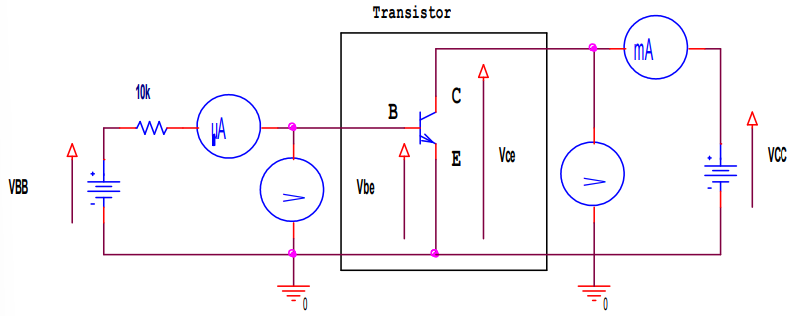
\includegraphics[width=0.75\linewidth]{Immagini/EXP6 - IV BJT.png}
        \caption{circuito per la I-V del BJT.}
        \label{fig: EXP6 - IV BJT}
    \end{figure}
    \item per evitare che le caratteristiche siano compromesse dall'aumento della temperatura del transistor è necessario limitare la potenza dissipata. A tal fine è necessario disegnare, prima di iniziare le misure, la curva di massima potenza: $P_{max} = V_{ce}I_c$ che nel piano $I_c = f(V_{ce})$ è rappresentata da un iperbole. Il transistor del laboratorio è del tipo NPN con sigla TIP31 e può dissipare al massimo $\SI{1}{\watt}$;
    \item variando $V_{be}$ tramite $V_{bb}$, impostare una corrente di base di $\SI{100}{\micro\ampere}$;
    \item leggere la tensione $V_{be}$;
    \item variare la tensione $V_{ce}$ (registrarla) tramite $V_{cc}$ e leggere la corrente $I_c$. Annotarsi la corrente $I_b$ e la tensione $V_{be}$ ad ogni variazione di $V_{ce}$. Se la corrente $I_b$ dovesse variare per un certo valore di $V_{ce}$ (quando si passa da regione di saturazione a regione attiva) non reimpostare $V_{be}$.
    \item si ripete la procedura variando la corrente $I_b$ da $\SI{100}{\micro\ampere}$ a $\SI{400}{\micro\ampere}$ a passi di $\SI{50}{\micro\ampere}$, così da ricavare la famiglia di curve $I_c=f(V_{ce})$ per $I_b=costante$;
    \item si ricavi inoltre la famiglia $I_b=f(V_{be})$ con $V_{ce}=costante$ e $\beta_f=I_c/I_b=f(I_c)$ per $V_{ce}=\SI{6}{\volt}$;
    \item si ricavi infine la tensione di Early effettuando una regressione lineare delle curve $I_c=f(V_{ce})$ nella regione attiva.
\end{enumerate}

\setcounter{section}{0}
\renewcommand\thesection{\Alph{section}}

\section{Effetto Early}
L'effetto Early si riferisce alla variazione di $I_c$ con la variazione della tensione $V_{ce}$, anche quando $I_b$ è costante. Idealmente, ci si aspetterebbe che $I_c$ sia indipendente da $V_{ce}$ nella regione attiva del BJT, ma in pratica $I_c$ tende ad aumentare con $V_{ce}$. Questo avviene perché l'area della regione base-collettore si riduce leggermente con l'aumentare di $V_{ce}$, riducendo la probabilità di ricombinazione e quindi provocando un aumento di $I_c$.

La tensione di Early $V_A$ è un parametro che quantifica l'effetto Early. Può essere interpretata come il valore ipotetico di $V_{ce}$ per cui $I_c$ si annullerebbe. La tensione di Early è normalmente negativa dato che l'inclinazione delle rette $I_c=f(V_{ce})$ è molto contenuta.
\chapter{Amplificatore}

\textbf{Obiettivo:} amplificare una tensione sinusoidale tramite un amplificatore ad un transistor ad emettitore comune e caratterizzare il fattore di amplificazione.

\paragraph{Strumentazione:}
\begin{enumerate}
    \item un generatore di tensione e un generatore di funzioni;
    \item un transistor BJT;
    \item due resistenze $R_b=\SI{5}{\kilo\Omega}$ e $R_c=\SI{50}{\Omega}$ (dorata);
    \item un oscilloscopio. 
\end{enumerate}

\paragraph{Procedura:}
\begin{enumerate}
    \item costruire il circuito;
    \begin{figure}[h]
        \centering
        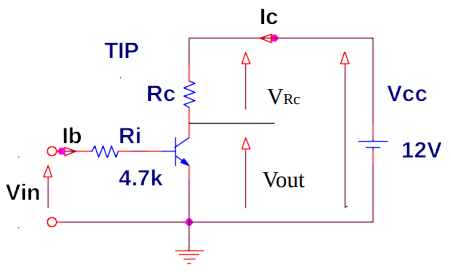
\includegraphics[width=0.55\linewidth]{Immagini/EXP7 - amplificatore.png}
        \caption{amplificatore BJT.}
        \label{fig: EXP7 - amplificatore}
    \end{figure}
    \item collegare in ingresso il generatore di funzione impostato su un'onda quadra di frequenza $\SI{1}{\kilo\hertz}$ e di ampiezza di qualche centinaia di mV sovrapposta ad un offset, questo deve essere tale si abbia $V_{ce}=\SI{6}{\volt}$ per $I_b$ costante;
    \item sovrapporre alla tensione di offset un'onda quadra molto piccola equivale a dare degli incrementi ad $I_b$. Ricavare con misure eseguite con l'oscilloscopio gli incrementi di $I_b$ e $I_c$
    \begin{equation}
        \Delta I_b=\frac{\Delta V_i}{R_i},\quad\Delta I_c=\frac{\Delta V_{ce}}{R_c},
    \end{equation}
    il cui rapporto fornisce
    \begin{equation}
        \beta_0=\left|\frac{\Delta I_c}{\Delta I_b}\right|;
    \end{equation}
    \item applicare un segnale sinusoidale e dal rapporto fra le ampiezze $V_{in}$ e $V_{out}$ lette sull'oscilloscopio calcolare l'amplificazione in tensione del segnale
    \begin{equation}
        A_V=\frac{V_{out}}{V_{in}},
    \end{equation}
    e verificare se è compatibile con il valore 
    \begin{equation}
        A_V=\frac{R_c}{R_i}\beta_0;
    \end{equation}
    \item Cambiare la frequenza di pilotaggio del segnale $V_{in}$ in ingresso e graficare $A_V$ in funzione della frequenza;
    \item Effettuare una regressione utilizzando come forma funzionale la funzione ricavata per il passa basso, aggiungendo un parametro che tenga conto del termine di amplificazione (guadagno maggiore di 1).
\end{enumerate}

\paragraph{Amplificazione di un'onda sonora (opzionale).} Collegare in parallelo alla resistenza $R_c$ un altoparlante e, mandando segnali di frequenza di circa $\SI{1}{\kilo\hertz}$, sentire l'onda sonora che si genera. Si può aumentare la frequenza fino alla frequenza di taglio dell'orecchio umano. Modulare il segnale in frequenza con lo sweep del generatore di funzioni e ascoltare l'onda sonora modulata.

\paragraph{Transistor in saturazione e interdizione (opzionale).} Osservare l'aumento della distorsione della tensione sinusoidale aumentando la tensione del segnale di ingresso fino ad avere il transistor in saturazione e in interdizione. Sostituire la $R_c$ con una lampadina e, facendo lavorare il transistor in saturazione ed interdizione, osservare che la lampadina si accende e si spegne (ovviamente se le frequenze di pilotaggio del transistor sono inferiori a $\SI{10}{\hertz}$).
\chapter{Cella solare}

\renewcommand\thesection{\Roman{section}}

\section{Rendimento di una cella solare}

\textbf{Obiettivo:} misurare l'efficienza di conversione fra l'energia elettrica prodotta da una cella solare e l'energia luminosa incidente.

\paragraph{Strumentazione:} 
\begin{enumerate}
    \item una cella solare;
    \item un banco ottico;
    \item un amperometro e un voltmetro. 
\end{enumerate}

\paragraph{Procedura:}
\begin{enumerate}
    \item disporre la cella sul banco ottico, il più possibile vicino alla lampadina, misurare la distanza pannello–filamento ed il diametro del pannello.
    \item costruire i circuiti: quello di sinistra è composto da un alimentatore di tensione continua in grado di fornire la potenza necessaria per alimentare la lampadina alogena;
    \begin{figure}[h]
        \centering
        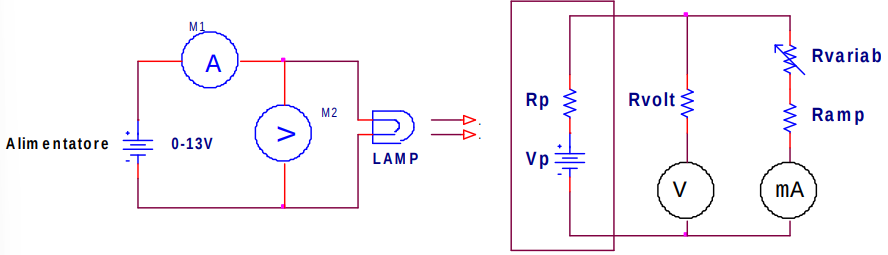
\includegraphics[width=0.9\linewidth]{Immagini/EXP8 - cella solare.png}
        \caption{circuiti per la lampadina alogena e la cella solare.}
        \label{fig: EXP8 - cella solare}
    \end{figure}
    \item alimentare la lampadina a $V_{gen}=\SI{12}{\V}$, leggere sul generatore di tensione in continua (o sul trasformatore) la corrente $I_{gen}$ che assorbe e la tensione e calcolare la potenza.
    \item effettuare le misure in avvicinamento;
    \item leggere la corrente $I$ indicata dal milliamperometro e la tensione $V$ sul voltmetro. Il rapporto fra tensione e corrente fornisce il valore della resistenza interna del milliamperometro, che non cambia, a meno di non cambiare scala allo strumento; in questo caso è necessario ripetere la misura;
    \item scollegare l'amperometro e leggere la tensione indicata: essa rappresenta la tensione $V_p$;
    \item osservare che la resistenza interna del pannello è di ordini di grandezza più piccola della resistenza del voltmetro;
    \item calcolare la resistenza $R_p$ della cella con i dati misurati di $V_p$, $I$ e $R_{amp}$;
    \item ricavare la corrente di cortocircuito della cella con $I_{cc}=V_p/R_p$;
    \item ricavare la potenza elettrica prodotta dalla cella con $P_{pannello}=I_{cc}V_p$;
    \item oscurare la luce che prodotta dalla lampada alogena incide direttamente sul pannello e misurare la potenza prodotta dalla luce di fondo $P_{fondo}$, ripetendo le misure da 4. a 8., la potenza generata dalla luce incidente sarà $P_{diretta}=P_{pannello}-P_{fondo}$;
    \item ripetere le misure da 4. a 9. per circo 10-15 distanze a intervalli di circa $\SI{5}{cm}$ l'una dall'altra e trovare la relazione tra l'efficienza e la distanza lampadina-pannello;
    \item graficare la corrente $I_{cc}$ e la tensione $V_p$ in funzione della distanza. Proporre un modello per interpretare i dati.
\end{enumerate}

\section{Caratteristica I-V di una cella solare}

\textbf{Obiettivo:} verificare il teorema del massimo trasferimento di potenza tramite l'aggiunta di un reostato e determinare la caratteristica I-V della cella.

\paragraph{Strumentazione:}
\begin{enumerate}
    \item un reostato;
    \item gli elementi della parte precedente.
\end{enumerate}

\paragraph{Procedura:}
\begin{enumerate}
    \item disporre la cella a una certa distanza dalla lampadina, non troppo vicina per evitare effetti termici (noi avevamo scelto il più lontano possibile);
    \item ATTENZIONE! Prima di procedere calcolare $R_{amp}$ e $R_{p}$ e assicurarsi che $R_p>R_{amp}$;
    \item determinare il range della resistenza di carico $R_{var}$;
    \item ripetere le misure da 4. a 8. (della parte I) facendo variare $R_{var}$;
    \item non è necessario fare le misure in oscuramento e si può fare un'unica misura di $V_p$ (step 5. della parte I);
    \item graficare la caratteristica $I(V)$ della cella;
    \item graficare la potenza fornita al carico (composto dalla $R_{var}$ e dalla resistenza $R_{amp}$). Se il modello proposto è corretto dovrà risultare un massimo della potenza trasferita per $R_p=R_{var}+R_{amp}$.
\end{enumerate}

\setcounter{section}{0}
\renewcommand\thesection{\Alph{section}}

\section{Considerazioni geometriche}
Per calcolare l'efficienza di conversione della cella elementare è necessario calcolare il rapporto fra la potenza incidente sulla cella e la potenza elettrica prodotta dal pannello. La potenza incidente sul pannello è ricavabile dall'angolo solido $\Omega$ sotteso dal pannello solare. Dato che
\begin{equation}
    \Omega=\int_{0}^{2\pi}d\phi=\int_{0}^{\theta}\sin{(\alpha)}\,d\alpha=2\pi(1-\cos{\theta}),
\end{equation}
e che la lampadina emette su tutto l'angolo solido di $4\pi$, la potenza che arriva sul pannello è la frazione $\Omega/4\pi$, quindi
\begin{equation}
    P_{incidente}=\frac{1-\cos{\theta}}{2}P_{lampadina},\quad P_{lampadina}=I_{gen}V_{gen}.
\end{equation}
Indicando con $r$ il raggio del pannello si può scrivere
\begin{equation}
    \cos{\theta}=\frac{d}{\sqrt{r^2+d^2}}.
\end{equation}
L'efficienza del pannello, in funzione della distanza $d$, è
\begin{equation}
    \eta=\frac{P_{diretta}}{P_{incidente}}.
\end{equation}
Nel caso in cui la sorgente luminosa è molto
distante dai pannelli, è possibile semplificare le relazioni tra potenza incidente e potenza prodotta approssimando la superficie del pannello ad una calotta sferica. In questo caso se $r\ll d$ si può approssimare
\begin{equation}
    \cos{\theta}=\frac{d}{\sqrt{r^2+d^2}}\approx 1-\frac{1}{2}\frac{r^2}{d^2}.
\end{equation}

\end{document}
